\documentclass[12pt, a4paper]{article}


\usepackage[utf8]{inputenc}  
\usepackage[T1]{fontenc}     
\usepackage[portuguese]{babel}


\usepackage{mathptmx}     


\usepackage{geometry}
\geometry{top=3cm, left=3cm, bottom=2cm, right=2cm}


\usepackage{setspace}
\onehalfspacing         


\usepackage{indentfirst}       
\setlength{\parindent}{1.25cm} 


\usepackage{graphicx}
\usepackage{url}


\usepackage{amsmath, amssymb}


\usepackage[hidelinks]{hyperref} 

\begin{document}

\begin{titlepage}
    \centering

    
\includegraphics[width=0.2\textwidth]{ufs-logo.png}\par\vspace{0.6cm}

    {\scshape\LARGE Universidade Federal de Sergipe \par}
    \vspace{0.3cm}

    {\scshape\Large Departamento de Computação \par}
    \vspace{1cm}

    {\scshape\large Disciplina: Processamento de Imagens\par}
    \vspace{2cm}

    {\huge\bfseries PreOCR: Detecção de Colunas, Linhas e Palavras em Imagens Binárias\par}
    \vspace{2cm}

    {\large\bfseries Discentes (Grupo 13):\par}
    \vspace{0.2cm}
    {\large Evandro José dos Santos Neto\par}
    {\large Gabriel Rodrigues dos Santos\par}
    {\large Gustavo de Jesus Rodrigues\par}
    {\large João Felipe Tunes Oliveira\par}

    \vspace{2cm}
    {\large\bfseries Docente:\normalfont\large\ Beatriz Trinchao Andrade de Carvalho\par}

    \vfill
    {\large Julho de 2026\par}
\end{titlepage}

\renewcommand{\contentsname}{\centering Sumário}
\tableofcontents
\newpage

\section{INTRODUÇÃO}
Este trabalho apresenta o PreOCR, um programa que recebe pela linha de comando uma imagem binária no formato PBM ASCII (tipo P1) contendo um texto com uma ou mais colunas, e retorna no terminal a quantidade de colunas, linhas e palavras desse texto. O programa também gera duas imagens de saída: uma versão filtrada da entrada, sem o ruído sal e pimenta, e uma versão em que cada palavra aparece circunscrita por um retângulo. Um sistema desse tipo corresponde à etapa de segmentação que antecede o reconhecimento óptico de caracteres (OCR), na qual as regiões da imagem que contêm palavras são localizadas antes de qualquer tentativa de identificação das letras \cite{b1}.

O programa foi escrito em Python, usando apenas a biblioteca padrão da linguagem. Todas as funções de processamento de imagens foram implementadas pelo grupo, sem o uso de bibliotecas prontas como OpenCV, NumPy ou Pillow. As técnicas aplicadas vêm das aulas de Morfologia Matemática da disciplina, que tratam a imagem binária como um conjunto de pontos em $\mathbb{Z}^2$ e a manipulam com operações entre esse conjunto e um elemento estruturante \cite{b1, b2}. Adotamos a convenção vista em aula, em que o valor 1 representa o pixel preto (texto) e o valor 0 representa o pixel branco (fundo).

Além do programa, foram criadas três imagens de teste de autoria do grupo, nomeadas no formato pedido na especificação, e o conjunto foi validado sobre as dez imagens da base de teste disponibilizada no SIGAA.

\section{TÉCNICAS APLICADAS}

\subsection{Leitura e escrita do formato PBM}
O PBM ASCII é um formato de imagem binária sem compressão, composto por um cabeçalho com o número mágico P1, a largura e a altura, seguido pelos valores 0 e 1 dos pixels \cite{b3}. O leitor implementado remove os comentários iniciados por \texttt{\#}, aceita os bits escritos juntos ou separados por espaços e valida o arquivo por completo: formato, dimensões, quantidade de pixels e valores permitidos. Qualquer problema gera uma mensagem de erro clara para o usuário.

\subsection{Remoção do ruído sal e pimenta}
O enunciado garante que o ruído tem o tamanho de um pixel. Um pixel preto isolado é detectado pela transformada hit-or-miss \cite{b1}, com o elemento estruturante composto pela origem (objeto) e pela vizinhança-8 (fundo). A remoção corresponde à operação de afinamento, $A \otimes B = A - (A \circledast B)$. O caso do pixel branco isolado dentro de uma letra é o dual, resolvido pelo espessamento, que preenche o buraco.

Nas imagens com ruído mais denso da base de teste, observamos que pixels de ruído vizinhos formam pares e trincas que a transformada de pixel isolado não alcança. Para removê-los, aplicamos uma erosão por um quadrado $2 \times 2$, que gera um marcador: como os traços das letras têm espessura de pelo menos 2 pixels, o marcador sobrevive somente dentro do texto verdadeiro, e os aglomerados de ruído desaparecem. Em seguida, a extração de componentes conexos a partir das sementes do marcador, dada pela iteração $X_k = (X_{k-1} \oplus B) \cap A$ até a estabilização \cite{b1, b2}, reconstrói apenas os componentes que contêm texto. Verificamos que nenhum componente legítimo da base de teste é perdido nesse processo. Consideramos usar uma abertura para essa etapa, mas ela danificaria os traços finos das letras, que têm espessura próxima do tamanho do elemento estruturante.

\subsection{Segmentação de palavras, linhas e colunas}
A ideia central da segmentação é que o espaço entre letras de uma mesma palavra é bem menor que o espaço entre palavras, que por sua vez é bem menor que o corredor entre colunas. Um fechamento $A \bullet B = (A \oplus B) \ominus B$ com elemento estruturante em reta horizontal, com raio proporcional ao tamanho da letra, funde as letras de cada palavra sem fundir palavras vizinhas. Essa estratégia de suavização por varredura é semelhante à usada em sistemas clássicos de análise de documentos \cite{b4}. Um segundo fechamento, com elemento em reta vertical de raio 2, une o pingo do i e do j ao corpo da palavra. Depois disso, cada palavra vira um único componente conexo, e a contagem é feita pela extração de componentes conexos vista em aula.

Para as colunas, um fechamento horizontal maior une as palavras de cada linha sem atravessar o corredor entre colunas, e uma dilatação vertical com elemento do tamanho da altura da imagem funde todas as linhas de uma mesma coluna em um único bloco. Como essa dilatação é puramente vertical, colunas distintas nunca se unem. As linhas são contadas dentro da faixa de cada coluna: uma dilatação horizontal seguida da interseção com a máscara da coluna transforma cada linha do texto em uma faixa conexa, e basta contar as faixas. Com isso, linhas de colunas diferentes contam separadamente, como pede a especificação.

Os retângulos da imagem de saída são as caixas delimitadoras dos pixels de texto de cada componente palavra, com uma margem de 2 pixels. Como o texto filtrado é subconjunto do seu fechamento, propriedade vista em aula \cite{b1}, os rótulos dos componentes fundidos podem ser usados diretamente sobre os pixels originais.

\subsection{Parâmetros}
Todos os raios são calculados em relação à altura mediana $h$ dos componentes conexos da imagem filtrada, estimada da própria imagem. Assim o programa funciona para qualquer corpo de fonte, sem valores fixos em pixels. Os parâmetros usados foram: raio do fechamento de palavras igual a $0{,}22 \cdot h$, raio do fechamento vertical do pingo igual a 2, raio do fechamento de linhas igual a $1{,}0 \cdot h$ e margem dos retângulos igual a 2 pixels. Na base de teste, $h$ ficou em torno de 18 pixels.

\section{PRINCIPAIS PROBLEMAS E SOLUÇÕES}
O primeiro problema encontrado foi o dos pingos de i e j e dos sinais de pontuação, que viravam palavras separadas (havia 368 componentes de altura 3 na base de teste). Medimos o vão vertical entre o pingo e o corpo da letra, que é de 3 pixels, e resolvemos com o fechamento vertical de raio 2, que une o pingo à palavra sem alcançar a linha vizinha.

O segundo problema foi o ruído denso, que forma pares e trincas de pixels. Após o hit-or-miss de pixel isolado ainda restavam 1.315 aglomerados na imagem \texttt{lorem\_s12\_c03\_noise}. A solução do marcador por erosão $2 \times 2$ com reconstrução por componentes conexos, descrita na seção anterior, eliminou todos sem perder nenhuma letra.

O terceiro problema apareceu nas variantes justificadas e com espaços vazios da base. Os espaços esticados do texto justificado quebravam a contagem de linhas, e os espaços vazios dividiam uma coluna em vários blocos. A solução foi contar as colunas com uma dilatação puramente vertical, que é insensível a vãos verticais, e contar as linhas por faixas horizontais dentro da máscara de cada coluna, o que é insensível ao espaçamento horizontal.

Também tratamos com cuidado as bordas das operações morfológicas. Pela dualidade $(A \ominus B)^c = A^c \oplus \hat{B}$, o complemento de $A$ em $\mathbb{Z}^2$ é infinito, então o que está fora da imagem conta como fundo na erosão. No fechamento, a dilatação intermediária é calculada com o domínio estendido, para não violar a propriedade $A \subseteq A \bullet B$.

Por fim, a eficiência. A dilatação e a erosão unidimensionais foram implementadas em tempo $O(N)$ por varredura dupla, medindo a distância de cada pixel ao objeto mais próximo, o que independe do raio do elemento estruturante. A extração de componentes conexos usa uma fila e visita cada pixel uma única vez, sendo a realização eficiente da definição iterativa da aula. Uma página A4 (1653 por 2338 pixels) é processada em cerca de 10 a 15 segundos em Python puro.

\section{RESULTADOS}
O gabarito de palavras foi extraído dos arquivos \texttt{.odt} que acompanham a base de teste. As contagens do programa foram exatas nas dez imagens, incluindo todas as versões com ruído, como mostra a Tabela \ref{tab:resultados}.

\begin{table}[h]
\centering
\caption{Resultados nas imagens da base de teste (com e sem ruído).}
\label{tab:resultados}
\begin{tabular}{lccc}
\hline
\textbf{Imagem} & \textbf{Colunas} & \textbf{Linhas} & \textbf{Palavras} \\
\hline
lorem\_s12\_c02 & 2 & 99 & 583 \\
lorem\_s12\_c02\_espacos & 2 & 81 & 476 \\
lorem\_s12\_c02\_just & 2 & 99 & 583 \\
lorem\_s12\_c03 & 3 & 150 & 557 \\
lorem\_s12\_c03\_just & 3 & 150 & 557 \\
\hline
\end{tabular}
\end{table}

O texto justificado tem exatamente as mesmas quebras de linha do texto não justificado (99 linhas nas duas versões de duas colunas e 150 nas de três colunas), o que confirma a contagem de linhas. As três imagens de autoria do grupo também retornam exatamente os valores presentes nos nomes dos arquivos: 1 coluna, 13 linhas e 108 palavras na primeira; 2 colunas, 38 linhas e 170 palavras na segunda; 3 colunas, 61 linhas e 223 palavras na terceira.

As Figuras \ref{fig:ruido}, \ref{fig:filtrada} e \ref{fig:palavras} mostram um recorte de uma das imagens da base: a entrada com ruído, o resultado da filtragem e a saída final com as palavras circunscritas.

\begin{figure}[h]
\centering
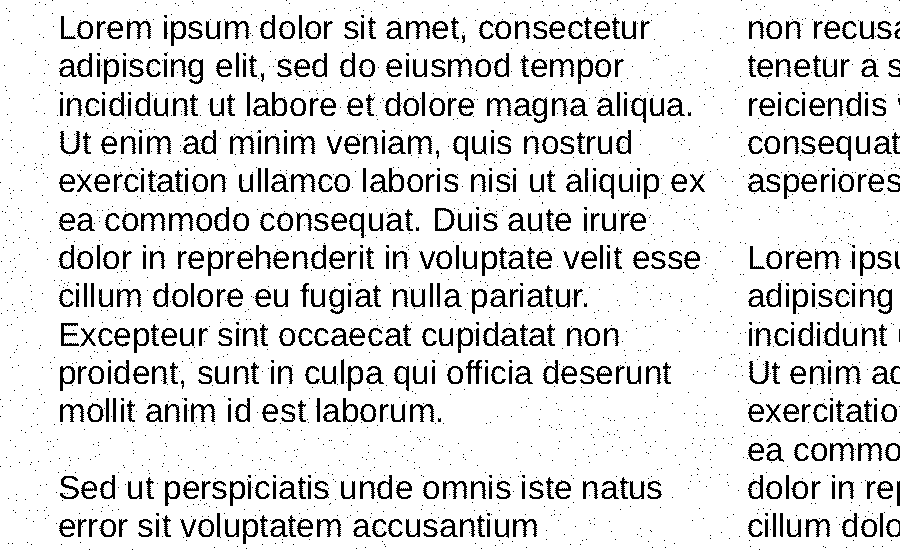
\includegraphics[width=0.85\textwidth]{fig1_ruido.png}
\caption{Recorte da imagem de entrada com ruído sal e pimenta.}
\label{fig:ruido}
\end{figure}

\begin{figure}[h]
\centering
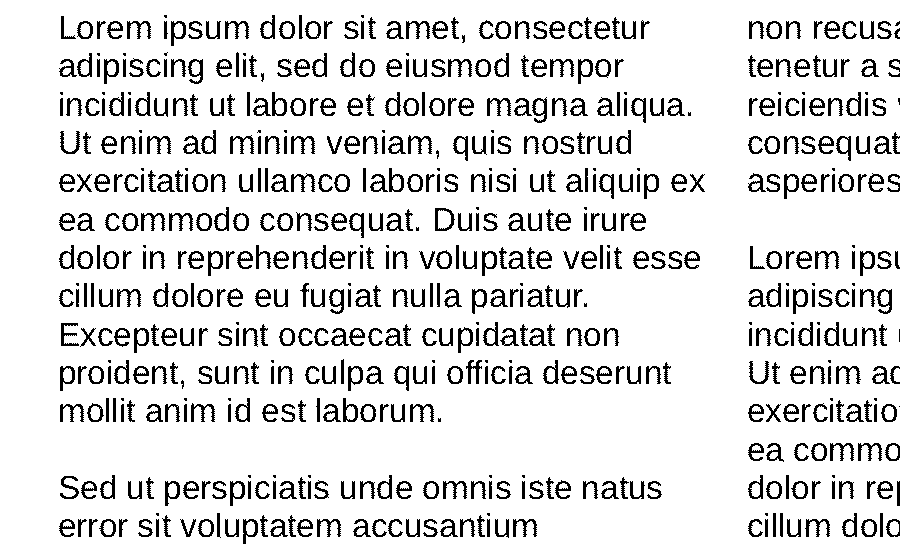
\includegraphics[width=0.85\textwidth]{fig2_filtrada.png}
\caption{Mesmo recorte após a remoção do ruído.}
\label{fig:filtrada}
\end{figure}

\begin{figure}[h]
\centering
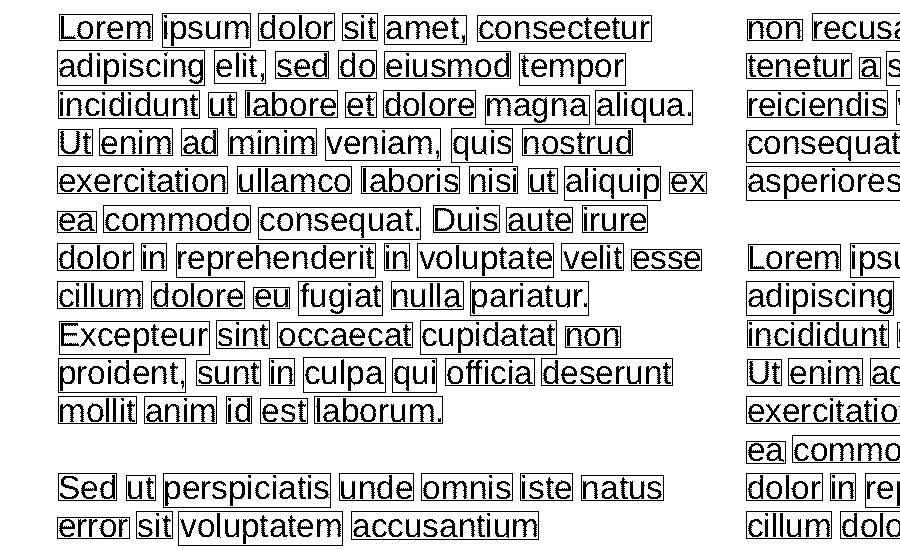
\includegraphics[width=0.85\textwidth]{fig3_palavras.png}
\caption{Saída final, com cada palavra circunscrita por um retângulo.}
\label{fig:palavras}
\end{figure}

\section{OUTROS TIPOS DE FONTE}
Verificamos o comportamento do programa com textos escritos em fontes diferentes da Arial. Geramos imagens de teste nas fontes Times New Roman (serifada) e Verdana (sem serifa) e o programa retornou as contagens exatas nas duas, sem a alteração de nenhum parâmetro. Isso acontece porque todos os raios são relativos à altura mediana da letra, estimada da própria imagem, e porque a proporção entre o espaço de letras e o espaço de palavras se mantém nas fontes proporcionais. As imagens desses testes estão na pasta \texttt{extras} do projeto.

Identificamos, porém, uma limitação com fontes monoespaçadas, como a Courier. Nelas, cada caractere ocupa uma célula de largura fixa, então o espaço entre letras se aproxima do espaço entre palavras e o fechamento com raio proporcional deixa de separar bem os dois casos. Uma extensão natural do trabalho seria estimar o limiar de fusão pela análise do histograma dos vãos horizontais de cada linha, em vez de usar uma proporção fixa da altura da letra.

\section{TRATAMENTO DE ERROS}
O programa rejeita, com mensagem clara no terminal: arquivo inexistente ou ilegível, formato diferente de P1, cabeçalho incompleto, dimensões inválidas, arquivo truncado e valores de pixel diferentes de 0 e 1. Uma imagem válida sem nenhum texto retorna 0 colunas, 0 linhas e 0 palavras, e as imagens de saída são geradas normalmente.

\section{COMPILAÇÃO E EXECUÇÃO}
O programa não requer compilação nem instalação de dependências, apenas o interpretador Python 3 (versão 3.6 ou superior), presente por padrão nas principais distribuições Linux. Para executar:

\begin{verbatim}
python3 PreOCR.py lorem_s12_c02.pbm
\end{verbatim}

A saída no terminal informa as contagens:

\begin{verbatim}
colunas: 2
linhas: 99
palavras: 583
\end{verbatim}

Os arquivos \texttt{lorem\_s12\_c02\_filtrada.pbm} e \texttt{lorem\_s12\_c02\_palavras.pbm} são gravados no mesmo diretório da imagem de entrada.

\newpage
\phantomsection
\addcontentsline{toc}{section}{REFERÊNCIAS}
\renewcommand{\refname}{\centering REFERÊNCIAS}
\begin{thebibliography}{00}

\bibitem{b1}
GONZALEZ, R. C.; WOODS, R. E. \textbf{Processamento digital de imagens}. 3. ed. São Paulo: Pearson Prentice Hall, 2010.

\bibitem{b2}
PEDRINI, H.; SCHWARTZ, W. R. \textbf{Análise de imagens digitais: princípios, algoritmos e aplicações}. São Paulo: Thomson Learning, 2008.

\bibitem{b3}
POSKANZER, J. \textbf{PBM Format Specification}. Netpbm documentation. Disponível em: \url{https://netpbm.sourceforge.net/doc/pbm.html}. Acesso em: 4 jul. 2026.

\bibitem{b4}
WONG, K. Y.; CASEY, R. G.; WAHL, F. M. Document Analysis System. \textbf{IBM Journal of Research and Development}, v. 26, n. 6, p. 647-656, 1982. DOI: \href{https://doi.org/10.1147/rd.266.0647}{10.1147/rd.266.0647}.

\end{thebibliography}

\end{document}
